\documentclass[12pt, abstracton]{article}
% 12pt als Standardschrift bedeutet \footnotesize ist in 10pt
\usepackage[utf8]{inputenc}
\usepackage[T1]{fontenc}
\usepackage{lmodern}
\usepackage[pdftex]{graphicx}
\usepackage{url}
% Package for quotes like in the Statutory Declaration
\usepackage{quoting}
\usepackage{amsmath, latexsym}
\usepackage{paralist} 
\usepackage{setspace}
% Normaler Abstand 1.1, bleibt bei Fussnoten erhalten, \doublespacing Zeilenabstand 1.5
% Packages for tables
\usepackage{longtable}
\usepackage{booktabs}
\usepackage{dcolumn}
% Set the spaces
\usepackage[left=4cm, right=3cm, top=3cm, bottom=3cm]{geometry}
% Special packages for graphics
\usepackage{epstopdf}
\usepackage {subfigure}
\usepackage{pgf,tikz}
\usetikzlibrary{trees}
\usetikzlibrary{arrows}
% Package for abbreviations
%\usepackage[printonlyused]{acronym}

% Bibliography mit Bibtex und natbib befehlen (siehe Dokumentation)
\usepackage{natbib}

\usepackage{caption}
\usepackage{makecell}
\usepackage{eurosym} % for Euro symbol
\usepackage{tabu} % for longtable (more than 1 page)
\usepackage{float}
\newcommand{\ra}[1]{\renewcommand{\arraystretch}{#1}}

\begin{document}

% % % % % % % % % % % % % % % % % % % % % % % % % % % % % %
% % % % % % % % % Title Page % % % % % % % % % % % % % % %
% % % % % % % % % % % % % % % % % % % % % % % % % % % % % %
\vspace*{2cm}
\begin{center}
\thispagestyle{empty}
\begin{spacing}{2}
{\LARGE Heterogeneous preferences for term life insurance: A latent class analysis for the segmentation of the population groups in Germany}\\[1.5cm]
\end{spacing}
{\bfseries \large Master Thesis}\\[11pt]
{supervised by the}\\[22pt]
{\bfseries \large Department of Economics}\\[11pt]
{\bfseries \large at the University of Zurich}\\[22pt]
{ Prof. Dr. Rainer Winkelmann}\\[11pt]
{ to obtain the degree of ''Master of Arts in Wirtschaftswissenschaften''}\\[3cm]
\begin{tabular}{ll}
\hline
Author: 			& Ulrich Schmid\\
Course of studies:  & Economics\\
Student ID: 		& 10-717-478\\
Address: 			& Bergacker 66\\
					& 8046 Zürich\\
Phone: 				& +41 76 369 16 47\\
E-Mail: 			& Ulrich\textunderscore Schmid@outlook.com\\
Date: 				& 20.04.2017\\
\hline
\end{tabular}\\[1.5cm]
\end{center}

% % % % % % % % % % % % % % % % % % % % % % % % % % % % % % % % % % % % %
% % % % % % % % % % % % % % % % Abstract % % % % % % % % % % % % % % % % %
% % % % % % % % % % % % % % % % % % % % % % % % % % % % % % % % % % % % %
\cleardoublepage
\pagestyle{plain}
\setcounter{page}{1}
\pagenumbering{roman}
\begin{abstract}
\footnotesize
This master thesis investigates whether there exist potential subgroups in the German population regarding their preferences for term life insurance contracts. By using a conditional logit model the average preferences of consumers regarding such contracts are estimated. Then, a latent class model is applied to identify diverse customer groups. The method is applied on a sample from an online survey conducted in 2013 by Swiss Re and the University of St. Gallen, where 3,181 participants have been asked about their preferences regarding different attributes of a term life insurance contract. In a first step, a latent class model without concomitant variables is applied. After that, a second model which uses demographic and sociodemographic variables as concomitant variables, is estimated.\\
The estimation suggests four subgroups. All of them show distinct patterns for certain product attributes. By considering the distributions of the sociodemographic variables of the groups, only cautionary statements can be made due to the fact that they appear to be very similar across the groups. The author concludes that on the one hand, there exists preference heterogeneity in the German term life market. These groups could be advertised strategically to attract new customer fields and enhance market shares for insurance companies willing to incorporate customer preferences into their strategies. On the other hand, no significant link between the preference variables and the demographic and sociodemographic variables could be found which leaves the question for future research if there is a way to find such a connection.\\
 \end{abstract}
% % % % % % % % % % % % % % % % % % % % % % % % % % % % % % % % % % % % %
% % % % % % % % % % % % Table of Contents % % % % % % % % % % % % % % % %
% % % % % % % % % % % % % % % % % % % % % % % % % % % % % % % % % % % % %
\cleardoublepage
\setcounter{tocdepth}{3}
\tableofcontents
\cleardoublepage
% Abbildungs- und Tabellenverzeichnis
\listoffigures
\listoftables
% List of Abbreviations
%\section*{List of Abbreviation}
%\begin{acronym}[Bash]
% \acro{SECO}{Staatssekreteriat für Wirtschaft}
% \acro{FED}{Federal Reserve}
%\end{acronym}
\cleardoublepage
% % % % % % % % % % % % % % % % % % % % % % % % % % % % % % % % % % % % %
% % % % % % % % % % % % % Main Part % % % % % % % % % % % % % % % % % % %
% % % % % % % % % % % % %% % % % % % % % % % % % % % % % % % % % % % % % %
% Set general preferences for the main part...
\pagenumbering{arabic}
\setcounter{page}{1}
\doublespacing
% % % % % % % % % % % % % % % % % % % % % % % % % % % % % % % % % % % % %
\section{Introduction}
Many people in the world choose not to insure themselves against the risk of pre-mature death. The reasons for this are manifold: Several surveys in the US, Latin America, Europe and Asia showed that the main motives why customers relinquish from buying life insurance products are the price, affordability and price-performance ratio. Other important aspects include the absence of need, the limited knowledge as well as the complexity of the product and also the lack of trust in the insurance industry (\cite{Kirova2013}, p. 2).\\
Many individuals today do not understand why they should buy term or life insurance in general. They do not even consider buying it. For a firm it is crucial to understand how they could differentiate their products in such a way that it attracts more consumers. Usually, pricing for life insurance products is constructed solely on a cost- and claims-based approach without taking into account customer needs. A shift from these approaches to a more universal process by inlcuding the preferences of customers could help to close the protection gap (\cite{Rischatsch2016}, p. 14).\footnote{The protection gap is a term which states how much the difference between the optimally insured and the actual insured amount in a market is.} By focusing more on consumers’ preferences and differentiate term life insurance products to their preferences instead of solely competing over price the insurance industry might be able to attract new customer fields (Braun et al. (2014), p. 1).\\ 
This thesis tries to shed light on what individuals care most about in a term life insurance contract. With a method called \textit{Latent class analysis} I try to identify different customer segments in terms of the respective product attributes of a term life insurance contract. Gathering deep information out of real purchase decisions for this product is hard since the offered products today are solely price- and cost-based and therefore there exists not much product variation. In 2013, Swiss Re outsourced the conduction of a survey to YouGov, a renowned market research company, where they asked 3,181 individuals in Germany about their preferences for term life insurance contracts. With the data from this survey the analysis will be carried out in this thesis. In addition to the existing literature of this market, this thesis tries to combine the preference variables with the demographic and sociodemographic variables of the individuals to see if there exist interrelations between them, i.e. if individuals with the same preferences also show similar patterns in their demographic and sociodemographic characteristics.\\
The remainder of this thesis is structured as follows. In Section 2, a brief definition of a term life insurance contract will be given and the concept of the willingness to pay will be introduced. Then, an overview of previous studies about preference analyses in life insurance markets will be presented. Section 4 discusses the methodology of the data collection, as well as the econometric model which is used to determine the distinct consumer segments. The results are contained in Section 5 and the final Section concludes the thesis.  
\cleardoublepage
\onehalfspacing
\section{Theoretical part}
\subsection{Term life insurance definition}
A term life insurance contract resembles a whole life insurance contract with the main difference that the period of its validity is changeable and that there usually comes no investment component with it (\cite{ABI2017}).\footnote{There is no cash-value accumulation as it is possible in a whole life insurance.}\\
 Coverage for such a contract comes at a defined term and a fixed premium rate. The most common ones used in Germany are 10, 15 or 20 years while the possible terms range from one to 50 years. Other components a term life insurance contract contains are the following:
 \begin{itemize}
 	\item Monthly premium rate
 	\item Underwriting process
 	\item Critical illness (CI) rider
 \end{itemize}
Most attributes in a term life insurance policy are variable, as example the critical illness cover which gives a payout if the insured person sickens on a pre-specified illness. Examples of diseases that might be covered, are: Certain types of cancer, multiple sclerosis, heart attacks or strokes. It is possible as well, that disabilities as a result of accidents or diseases will be covered. In such a case an additional payout to the mortality risk can be added.\\
Whereas the purpose of a life insurance policy is to cover the mortality risk, a term life insurance contract can be a valuable option for hedging a mortgage or a consumer credit (\cite{GablerWirtschaftslexikon2017}). Further options to close such a contract refer to house builders who want to secure the financing of their projects, families with only one principal earner or unmarried couples since they have no claim on a widow’s pension or annuity (\cite{GDV2017}).\\ 
Another important aspect is the calculation of the premiums for a specific contract. Following factors are usually considered when calculating them:
 \begin{itemize}
 \item Health status
 \item Amount of coverage
 \item	Duration
 \item	Actuarial age of entry
\end{itemize}
Insurance companies or the association of actuaries use so-called mortality tables to calculate the premiums, while separate tables for smokers and non-smokers are created (\cite{GDV2017}). There exist several forms of term life insurance contracts, for example renewable term insurance, where one can take out the need for any further evidence of health or convertible term insurance, where it is possible to convert the policy to a whole life insurance contract (\cite{ABI2017}).\\
The German market for term life insurance is well developed and competitive. The premium volume in 2015 was approximately EUR 4,210 million, where new business was EUR 351 million. 7.65 million policies were in force. Premium income from in-force business has been growing slowly since 1995 but as Figure \ref{fig:PolicyGE} shows, new sales were at a climax in 2006 and on the decline since without showing any sign of growing back (\cite{Braun2014}, p. 2).
\begin{figure}[H]
	\includegraphics[width=\textwidth]{"New Business Ge".jpg}
	\caption{No. of new policies of term life insurance in Germany.}
	\label{fig:PolicyGE}	
\end{figure}
This decline serves as an indicator that it has become more difficult for German insurance companies to acquire new customers. It is also a sign that competition on price, distribution channels and product design has intensified and therefore innovative methods to attract new customers could be of high value (Braun et al. (2014), p. 2).
\subsection{The concept of the willingness to pay}
Knowledge of individuals’ reservation prices or willingness to pay (further abbreviated as WTP) is crucial for any pricing decisions. By using a metric as the WTP the results of the later analysis gain more intuitive economic meaning. One can differentiate between the maximum WTP and the marginal willingness to pay (MWTP). Whereas the maximum WTP stands as a reservation price in whole products, the MWTP is used to describe the reservation price for changes in product attributes (\cite{Jedidi2009}, p. 39). Jedidi and Jagpal (2009, p. 38 – 39) define the maximum WTP as a consumer’s reservation price where he or she is indifferent between buying a product and not buying it. To illustrate this, let y be the income of a consumer who is considering a purchase of one unit of a product \textit{g} to a certain price \textit{p}. Let $U(g, y-p)$ be the utility function of the respective consumer. The consumer’s reservation price $R(g)$ is implicitly given by
\begin{align}
U(g,y-R(g)) - U(0,y) = 0
\end{align}
The MWTP on the other hand is defined as the marginal rate of substitution between non-price and price attributes.  Let us consider a utility function which is a linear function of the observed factors of a term life insurance contract. The mathematical representation looks as follows:
\begin{equation}
\begin{split}
U = b_{1} Premium + b_{2} Brand + b_{3} SalesChannel + b_{4} CIRider\\ + b_{5}Duration + b_{6} UnderwritingProcedure + \epsilon
\end{split}
\end{equation}
To get the MWTP for e.g. brand, take the partial differentials of the utility function with respect to the premium and brand where  
\begin{align}
dU/dPremium = \beta_{1}dPremium\\
dU/dBrand =  \beta_{2}dBrand
\end{align}
Build the ratio of them :
$\frac{dU/dPremium}{dU/dBrand}$
and solve for it. Then $\frac{dPremium}{dBrand} = -\frac{\beta_{2}}{\beta_{1}}$. Setting it to 0 means that utility is held constant, so we see what change in  brand is needed to keep utility for the individual at the same level if the premium is altered (\cite{Train2003}, p.47). Analogously, we can define the other marginal rates of substitutions for the other coefficients in our equation.\\
It is important to mention that this definition for the MWTP possesses some pitfalls. The utility function defined above is quasi-linear and strictly linear in price. Although this definition is consistent with utility theory, a consumer does not necessarily react linearly to price changes. Another problem might arise when individuals use the price coefficient as a sign for quality. Then, price has two opposing effects: It lowers the consumer's utility and at the same time it is used as a quality parameter. If the quality gain excels the utility loss from a higher price, the MWTP turns negative.
A further issue can be the case where an estimated price coefficient is extremely small for a consumer.\footnote{This can occur if the data is noisy or the consumer is insensitive to price changes.} Due to this, WTP coefficients might get unrealistically large. There are several ways to address such problems, for example to constrain the price coefficients for the individuals in order that lower prices always induce higher utilities (\cite{Jedidi2009}, p. 46 – 47). Another limitation of the WTP concept is, that it can not account for the possibility of not buying a product or introducing competition in the market of the product and it does not consider a specific product context as well (Braun et al. (2014), p. 9).
\cleardoublepage
\onehalfspacing
\section{Literature overview of preference analyses in the insurance market}
In an insurance context, several articles concerning the willingness to pay for health insurance, long-term care (LTC) or crop insurance can be found. For example, Jacobs-Lawson et al. (2010) try to assess whether certain demographic characteristics can be associated with being uninsured. Their results indicate that individuals who are poor, unhealthy or older are willing to pay less for health insurance than their counterparts. Another study by Costa-Font and Font (2009) tries to shed light on the fact that long-term care insurance is sold badly in Spain. They test the hypothesis if in general, human beings’ myopia in planning insurance can be confirmed or rejected. For this, they conduct a survey where they ask the participants if they were to buy a LTC insurance at their current age and in a next question they ask them if they were to buy at the age of 40. Only about a fifth of the individuals considers LTC insurance as a suitable option for them. Their findings demonstrate that the WTP does not differ significantly for the states of age but rather by the participants’ perceptions of their probability to survive. Sherrick et al. (2003) show in their paper about crop insurance which U.S. farmer prefers what kind of insurance type. In a conjoint analysis, they find that on the one hand farmers prefer flexibility regarding different types of insurance and also regarding the coverage level and that on the other hand demand is greater by larger and younger farmers and those who farm in separate locations.\\
A further study published by Swiss Re in 2013, tries to shed light on the fact that there exists an undercoverage in life insure contracts and shows that in Asian countries such as Malaysia, income has a significant influence on the WTP for such contracts. Whereas poor households are willing to pay a much smaller amount than rich participants, richer households additionally have a higher share of life insurance buyers (\cite{Kirova2013}, p. 27).\\
When looking explicitly for articles within a term-life insurance context, three studies were found. Two of them were solely published by the Institute of Insurance Economics of the University of St. Gallen (see Braun et al. (2014); Schreiber (2016)) and one was conducted collaboratively by Swiss Re and the IVW (\cite{Braun2014}). The one published by Swiss Re and the IVW was based on the study conducted by Braun et al. (2014) and had the same main findings and conclusion, so I will not go into detail with this study.\\
In the first paper by Braun et al. (2014) perform a choice-based conjoint analysis with the same data which is used in this master thesis. In their study, they show that the product attributes brand, critical illness cover and medical underwriting are the most important non-price attributes of a term life insurance contract. They also find that there is large discrepancy in the distribution of consumers' preferences who are interested in such insurance products. This supports the assumption of preference heterogeneity in the German population.\\ Their results suggest that a change from cost- to preferences-based pricing would not only benefit the seller of term life insurance contracts, i.e. the insurance firms, but also would help to close the protection gap and help the population in their financial planning.\\
In contrast to the more general assumption in my master thesis, Braun et al. (2014) assume that the preference parameters are normally distributed among the population whereas the estimation method I apply does not beforehand define the distribution of the preference parameters but decides during the maximization process which distribution fits the data best. They also note that just because for example a personal sales channel is preferred to an online one it would not make sense to sell every term life contract through a human salesperson. The gain in customers has to be balanced to the additional costs that a nation-wide network of local salesmen would cause for the company. The positive MWTP for a human sales person might be crowded out by the cost savings.  They suggest that companies which want to enter the German term life market should focus on offering other products than well-established insurance companies do. But they also note that there are a lot of individuals who do not need coverage for mortality risk and therefore not want to buy such a contract. A term life contract is only beneficial for them if there is a distinct security motive present since the policyholders do not get any payment out of it.\\
With the results they obtained from the preference distributions they constructed four term life insurance products to cover the distinct preferences:\\\\
1. A "budget" product, with a contract duration of 15 years, an online sales channel, an underwriting process of 10 questions and without a CI cover. The product would be sold by a non-insurance firm.\\
2. A "classic" product, with a contract duration of 15 years, a human sales person, a medical examination as an underwriting process and without a CI cover. The product would be sold by a well-known insurance firm.\\
3. An "innovative" product, with a contract duration of 15 years, an online sales channel, no medical underwriting but 1-year waiting period until the contract begins and with a CI cover. The product would be sold by an unknown insurance firm.\\
4. A "premium" product, with a contract duration of 15 years, a human sales person, an underwriting process of 3 questions and  a CI cover. The product would be sold by a well-known insurance firm.\\\\
With these products they perform a simulation for market shares and how they would fare when introducing them in the German term life market. In their results the highest profit for the budget, classic and innovative product could be attained when they try to gain the highest share in preferences. For their premium product a loss in buyers is compensated by the increased price level since there are enough consumers for the premium product who are less price sensitive. What they do not incorporate into their study is the generation of different customer segments, they solely generate the respective preference distributions for every product attribute and then directly build four different products out of their findings. A point they mention in the end but not investigate in their analysis is the inclusion of sociodemographic and demographic variables which will be done in this thesis.\\
The second paper which will be reviewed is the one by Schreiber (2016) called: Identification of Customer Groups in the German Term Life Market: A Benefit Segmentation. He runs a choice-based conjoint analysis and subsequently a hierarchical Bayes estimation on the same data set as Braun et al. (2014) in order to find part-worth utility profiles of the participants of the survey. He states that there exists considerable disagreement regarding the respondents’ preferences and therefore heterogeneity is present. After this, he runs several hierarchical and partitioning cluster analyses with various linkage criterions to find different preference segments of the respective participants. In a next step, they merge the results from these techniques into a cluster ensemble and it is subjected to a consensus clustering algorithm from the k-means family. Their solution suggests three clusters of consumers with different preference patterns: One market segment consists of price-sensitive individuals who have low preferences for the other product attributes. The second cluster exhibits participants who value the brand the most, so they prefer well-known and -established companies with a good reputation in the insurance market. They also care relatively much for the underwriting process of the insurance policy and the critical illness option of such a contract, whereas the monthly premium rate of the contract is less important to them. The last segment consists of customers who are in a middle place of the two other partitions. They have the most balanced relative attribute importances of the three clusters and therefore are named as waverers by Schreiber. They also consider the price of the contract as the most important attribute but to a lesser degree than the first segment. The individuals from the third group place a high importance to the underwriting policy, the critical illness option as well as the brand of the insurer. The attributes term and sales channel on the other hand seem to be of minor relevance to all groups.\\
Schreiber (2016) states that these results might be of major importance for term life insurance providers since it offers them strategies of how to gain new or existing consumers. For example, the first two segments can be accessed by brand as well as not well-known insurers. The well-known insurance firms can focus on the cluster which values the reputation of a firm a lot and the lesser known insurance providers can focus on the segment which cares about the premium level by a competitive price setting. The third group of customers offers a potential to attract new customers. By expanding their existing product portfolio to this third segment, insurance firms can enlarge their customer community. \\
Altough the authors of these studies apply several methods to concern their findings, they also point out that there does not exist one correct methodology on which cluster technique one should apply and therefore all the results have to be considered with caution. Nevertheless, their findings can serve as a good benchmark and it will be interesting to see if the results found by the IVW and Swiss Re can be supported by this thesis or if different findings will emanate.
\cleardoublepage
\onehalfspacing
\section{Methodology}
\label{Methodology}
When it comes to the methodology first the question has to be answered why an experiment has been conducted instead of evaluating real life decisions. This will be the content of Section 4.1. After the first part the experimental design and the composition of the sample used for the later analysis will be discussed. In the final subsection, Section 4.3, the econometric specification will be shown.
\subsection{What is a Choice-Based Conjoint Analysis and which advantages and disadvantages does it have?}
\label{cbc_analysis}
Choice-based conjoint analysis originated from the technique known as conjoint analysis, a term mainly used in the marketing literature. It is a method where individuals express their preferences by comparing paired products and state which product they prefer. They do not make a rating or ranking of all the articles but rather choose the one which they think suits best for their preferences (Sawtooth Software, 2013, p. 2). A choice-based conjoint analysis therefore belongs to the type of an indirect stated preference method and not a revealed or direct stated preference method. One of the first applications was provided by Green and Rao (1971) in the context of marketing research and more recently, it has been employed in several WTP studies (see e.g. Breidert et al. (2006)). This first application by Green and Rao (1971) could still be considered as a conjoint analysis and later \cite{Louviere1983} suggested the approach which is known as a choice-based conjoint analysis. Contemporarily, the economic literature reported new ways to model discrete choices. As a theoretical foundation they used the theory which is known as random utility theory(\cite{Kjaer2005}, p. 23). Louviere et al. (2000) argue that techniques based on random utility theory should be named discrete choice experiments instead of conjoint analysis in order to be able to distinguish between choice-based experiment that are used in economics, from different methods which are not based on economic theory.\\
 Whereas the first ratings and rank-ordered conjoint analysis are only evaluated in a non-competitive situation where the participant does not have to choose between complete product profiles, a choice-based conjoint analysis is characterized by a trade-off between different products and an opt-out option.\\
As every method a choice-based conjoint analysis exhibits various advantages as well as disadvantages which will be discussed in this subsection. The following arguments have been taken from Sawtooth Software (2013, p. 2-4).\\
One of the advantages is that it simulates what consumers actually do in a real market environment. The act of choosing out of several possibilities the preferred one is something everyone understands and it comes in as natural thing to do.
Another pro lies in the fact that it is possible to integrate an opt-out option in the design of the questionnaire. By including this option a participant can give additional information to the researcher about the decrease in demand if e.g. the prices of the showed product choices increased.\\
Usually, it is difficult to quantify interactions with a conjoint analysis. Since choice-based conjoint analyses are analyzed by pooling information across respondents, it is possible to measure interaction effects and not solely main effects. An example for such an interaction can be the brand and price attribute of a product. Such an interaction can be included in the experimental design without making it more complex.\footnote{Interaction effects are often present when there exists different preferences in groups or individuals. This might be of a lesser problem in this study because the method used here is to model groups with different preference parameters.} Those are some of the advantages of a choice-based conjoint analysis. Still, there exist also disadvantages which have to be kept in mind when conducting such an investigation.\\
Since the individuals make the choices there is always some sort of inefficiency present. One inefficiency lies in the fact that respondents usually have to process a vast amount of information when deciding on which product to choose since the choice sets they have to evaluate are described by all the attributes considered for the product and each choice set contains various alternatives. A consequence out of this is that the researcher obtains less information than he would have received if the respondents were asked to rate each alternative in the choice set.\\
Also, there is a limit to how many attributes of a product can be processed by the participants. \cite{Green1990} for example considered a maximum number of six attributes that can be handled with full-profile concepts in a conjoint analysis without being confounded or ending up ignoring some of the attributes.\\
To deliberate about whether the advantages or disadvantages overweigh in the case of applying a choice-based conjoint analysis for term life insurance it can be stated that the advantages overweigh the disadvantages. First, a term life insurance policy can be regarded as a infrequently-purchased, durable and rather abstract product category where a direct stated preference approach would result in generating inaccurate WTP estimates (Braun et al. (2014), p. 3). Among the indirect stated preference methods the CBC approach is in favor for price-related studies (\cite{Orme2009}).
\subsection{Experimental design and sample composition}
\label{exp_design}
A crucial part for the generation of the data for the later analysis is how to design the questionnaire and how to conduct the discrete choice experiment. Swiss Re and the Institute of Insurance Economic (University of St. Gallen) did a collaborative research project in 2014 (On Consumer Preferences and the Willingness to Pay for Term Life Insurance, 2014) where they determined the product attributes and levels for their CBC analysis. The way they came up with those was through focus group discussions with industry professionals. Through these, seven product attributes where chosen:
\begin{table}[H] \centering 
	\label{Premium_Levels} 
	\resizebox{\textwidth}{!}{\begin{tabular}{lll}
			\hline \\[-1.8ex]
			\textbf{Product attribute} &\textbf{Levels} & \textbf{Annotation} \\
			\hline \\[-1.8ex]  
			Brand of the insurer & Well-known insurer, lesser-known  & Pictures (logos) of respective firms \\
			& insurer, non-insurer & in survey \\
			& & \\
			Critical illness (CI) rider & with, without & Payout of 50,000 EUR if diagnosed  \\
			& & with pre-specified disease\\
			& & \\
			Duration of the contract & 10, 15 or 20 years & -\\
			& & \\
			Monthly premium rate & Very low, low, middle, high, & Premia differ by group (see Table 2) \\
			& very high & \\
			Sales channel & Online channel or human salesperson & - \\	
			& & \\
			Underwriting procedure & Medical examination, 3 questions, & - \\
			& 10 questions, one-year waiting period& \\
			& &\\
			Sum insured & Fixed at 100,000 EUR & - \\
			\hline		
	\end{tabular}}
	\caption{Product attributes of a term life insurance contract used in the study.} 
\end{table}
When assessing the appropriate levels for the premiums the guidelines from \cite{Orme2002} were used: 1. Concisely state the levels and do not use ranges (participants may interpret them differently). 2. Independence of the attributes used 3. Attribute levels should be mutually exclusive (e.g. when you have to use a single level from each attribute for the analysis). The range for the different premium rates were achieved by interviewing market experts and assessing quotes for a immense number of products through an online comparison website called www.check24.de. Another important point for the design of the term life insurance is that premiums differ according to age and health of an individual. For this reason, the survey participants were allocated to ten different groups that were defined through their age and smoking status. This was necessary to ensure that every participant faces a price range which matches her or his mortality risk. Therefore, every participant was matched to one of the groups showed in Table 2.\\
% Table created by stargazer v.5.2 by Marek Hlavac, Harvard University. E-mail: hlavac at fas.harvard.edu
% Date and time: Mo., Apr 03, 2017 - 11:36:01
% Requires LaTeX packages: dcolumn 
\begin{table}[!htbp] \centering 
	\label{Premium_Levels} 
	\resizebox{14.5cm}{4cm}{\begin{tabular}{@{\extracolsep{25pt}}D{.}{.}{-3} D{.}{.}{-3} D{.}{.}{-3} D{.}{.}{-3} D{.}{.}{-3} D{.}{.}{-3} }
		\hline \\[-1.8ex]
		\multicolumn{0}{l}{\textbf{Non-Smoker}} & \multicolumn{3}{c}{Price Levels (EUR)} \\
		\hline \\[-1.8ex]  
		\multicolumn{1}{l}{Age} & \multicolumn{1}{r}{Very Low} & \multicolumn{1}{r}{Low} & \multicolumn{1}{r}{Middle} & \multicolumn{1}{r}{High} & \multicolumn{1}{r}{Very High} \\
		\hline \\[-0.8ex]
		\multicolumn{1}{l}{20-29} & 3.00 & 6.00 & 9.00 & 12.00 & 15.00 \\
		\multicolumn{1}{l}{30-39} & 5.00 & 10.00 & 15.00 & 20.00 & 25.00 \\
		\multicolumn{1}{l}{40-44} & 7.00 & 14.00 & 21.00 & 28.00 & 35.00 \\
		\multicolumn{1}{l}{45-49} & 10.00 & 20.00 & 30.00 & 40.00 & 50.00 \\
		\multicolumn{1}{l}{50-54} & 20.00 & 40.00 & 60.00 & 80.00 & 100.00 \\	
		\hline \\[-0.8ex]
		\multicolumn{0}{l}{\textbf{Smoker}} & \multicolumn{3}{c}{Price Levels (EUR)} \\
		\hline \\[-0.8ex]  
		\multicolumn{1}{l}{Age} & \multicolumn{1}{r}{Very Low} & \multicolumn{1}{r}{Low} & \multicolumn{1}{r}{Middle} & \multicolumn{1}{r}{High} & \multicolumn{1}{r}{Very High} \\
		\hline \\[-0.8ex]
		\multicolumn{1}{l}{20-29} & 5.00 & 8.75 & 12.50 & 16.25 & 20.00\\
		\multicolumn{1}{l}{30-39} & 10.00 & 17.50 & 25.00 & 32.50 & 40.00\\
		\multicolumn{1}{l}{40-44} & 20.00 & 35.00 & 50.00 & 65.00 & 80.00\\
		\multicolumn{1}{l}{45-49} & 30.00 & 52.50 & 75.00 & 97.50 & 120.00\\
		\multicolumn{1}{l}{50-54} & 60.00 & 105.00 & 150.00 & 195.00 & 240.00\\
		\hline		
	\end{tabular}} 
	\caption{Premium Attribute Levels for different Age/Mortality Riks Groups} 
\end{table}
Policies were offered at terms of 10, 15 or 20 years assurance. This is a common range used in the industry. The underwriting procedures to determine the risk of a buyer for the insurance company could be assessed through different procedures. One was over a simple three-questions questionnaire, another over a ten-questions questionnaire. There was a third one which required the most effort via a medical examination and a newer one where no test or questionnaire was conducted but the insured person has a waiting period of one year until the contract comes into force. The attribute brand has three different specifications: One is that a well-known insurance company (e.g. Generali) offers the policy, another is that a rather unknown insurer (e.g. MyLife) is chosen and the third one is an option where a company which is not known for insurance contracts but is generally well-known (e.g. VW). The last attribute used is the critical illness rider option. By choosing this feature an individual gets a lump sum payout if the individual sickens with a defined illness as for example Cancer or multiple sclerosis during the contract term. The sum insured for the mortality risk remains unaffected by this option (Braun et al. (2014), p. 5–7).\\
When looking at the different attributes and the attribute levels that a term life insurance contract offers, it is apparent that it is not feasible to conduct a full factorial design for such choice tasks since there are too many possible contract combinations. The question is how many choice tasks a respondent should answer in order that enough information is gathered for a thorough analysis. For the survey used in this thesis, this procedure was outsourced to the firm YouGov which is a renown company for online market research. They incentivized people to participate by earning bonus points for online shops if they answered the questionnaire.\\
They conducted an online survey in 2013 and asked 3,181 German individuals about their opinion about term life insurance products.\footnote{For the final analysis only 2,145 participants were chosen, since the remaining ones did not fully answer all relevant questions for the experiment.} To ensure that approximately all 10 groups are equally represented, a ten percent quota was targeted (Braun et al. (2014)). Different to Braun et al. (2014), in this thesis all the observations were included in the analysis in order that more population representative statements can be made.\footnote{Braun et al. (2014) excluded all the participants from their estimations who did not identify themselves as term life insurance decision makers.}
The age of the participants ranged from 20 to 54 and was virtually population-representative according to domicile state and gender. This range in the age was chosen because most term life insurance policies are issued during the employment phase (\cite{Kirova2013}). In the beginning the participants were asked about their age, gender, self-perceived health status, education, profession, if they are smoker etc. After that, the hypothetical buying situation and how a term life insurance works were explained to the participants.\\
The study was designed as followed: Each respondent answered a hypothetical buying situation where two different term life insurance contracts where given to him or her. This was one choice set. In total every respondent answered 12 such choice sets. After choosing between the two contracts the respondents were asked if they would buy the product they had chosen before (i.e. opt-out decision) in order to make it more realistic and have further information about the product. After the survey the respondents answered additional questions which were posed to capture their views towards insurance and why they were in favor for buying or not buying such a product. The pairwise choice sets where generated according to the balanced overlap method, which is a randomized experimental design (Braun et al. (2014), p. 7). This method is the default option in Sawtooth Software and is nearly as efficient as the Complete Enumeration and Shortcut Methods in capturing main effects, but it outperforms the two other methods in measuring more precisely interaction effects (Sawtooth Software (2013), p. 17).\\ 
\subsection{Discrete choice models}
\label{DCEs}
To be able to explain how the participants value the different product attributes of a term life insurance contract two different models will be empirically applied. Since the dependent variable of choosing a term life contract offered in the experiment is binary, econometric literature suggests the usage of logit or probit models (See e.g. Boes and Winkelmann (2009); Train (2003)). I start with the conditional logit model before I refine the analysis and apply in a second stage the latent class probabilistic conjoint model to form customer segments. 
\subsubsection{The Conditional Logit model as a starting point}
\label{cond_logit}
The starting point for the analysis is the conditional logit model. It assumes that the individuals maximize their utility out of the choices they are encountered with at a time (Consistent with random utility theory, see e.g. \cite{Thurstone1927}). Their utility is defined via a indirect utility function, where individual i gets a utility from the term life insurance contract, j stands for the chosen alternative:\\
\begin{align}
Y_{ij}= \beta' X_{ij} + \epsilon_{ij}
\end{align}
\textit{$Y_{ij}$} stands for the utility which a respondent gets from choosing the respective term life insurance contract and \textbf{$\beta' X_{ij}$} is the deterministic part of utility explained by the attributes of the insurance product whereas \textit{$\epsilon_{ij}$} is the non-explained part of the utility. 
In our case the vector \textbf{$X_{ij}$} is defined as:
\begin{equation}
\begin{split}
\beta' X_{ij} & = \beta_{d15} Duration15_{ij} + \beta_{d20} Duration20_{ij} + \beta_{UW3} UW3Q_{ij}\\
& + \beta_{UW10} UW10_{ij} + \beta_{UWno} UWNON_{ij} + \beta_{online} Online_{ijc} \\
& + \beta_{Br2} Brand2_{ij}
+ \beta_{Br3} Brand3_{ij}
+ \beta_{CI} CIRider_{ij}
+ \beta_{P} Premium_{ij}
\end{split}
\end{equation}
\textit{Duration15} \& \textit{Duration20} stand for a contract with a term of 15 years respectively 20 years, \textit{UW3Q}, \textit{UW10Q} and \textit{UWNON} for an underwriting procedure of only three questions respectively 10 questions and no questions (but a freezing period of one year), \textit{Brand2} and \textit{Brand3} stand for a contract offered by a not so well-known german insurance firm respectively not a firm associated with selling insurance products (e.g. Aldi or VW), \textit{CIRider} stands for a contract which exhibits a Critical Illness option and \textit{Premium} stands for the monthly premium amount which has to be paid by the individual when buying a term life insurance contract.\\
From this equation we are also able to derive the willingness to pay (WTP) estimates of an individual for a specific product attribute by using the derivation from Section 2.2, where \textit{(-$\beta_{attribute}$/$\beta_{P}$)} defines the WTP of a certain product attribute for individual i. The WTP stands for the marginal euro value that an individual is willing to pay for a contract which exhibits e.g. the Critical illness rider option contrary to one without such a feature.\footnote{The confidence intervals generated with the function refit() with the program R will not be exactly correct because specific fitted models have already been determined using the same data (\cite{Gruen2008}, p. 18).}\\
Through several steps one can derive from equation (5) the choice probability of individual i choosing the alternative j in set c via the following probability function, consisting of the product attributes:
\begin{align}
\pi_{ij}= \frac{exp[\beta' X_{ij}]}{\sum_{k=1}^{J}{exp[\beta' X_{ij}]}}
\end{align}
\textit{$X_{ij}$ = Characteristics of alternative j}.\\
Whereas the conditional logit is a good starting point because of its relative simplicity it exhibits several shortcomings: First, it assumes independence of irrelevant alternatives. This means that the odds of any two outcomes are independent of the number and nature of other outcomes being simultaneously considered (Train, 2003). This can be tested e.g. via the Hausman ad Mcfadden IIA test (\cite{Hausman1984}). Second, it assumes that there exists no correlation between the error terms. This could be solved by taking a Probit instead of a Logit model while in the case of a Probit there still would be the assumption of a Gaussian distribution. The last important shortcoming is the one that a conditional logit assumes preference homogeneity among the individuals, i.e. that the preference parameters among the individuals, the betas, are the same. Several methods exist to overcome these aforementioned issues, where in this thesis a Latent Class Model will be used to mitigate these issues. 
\subsubsection{A latent class probabilistic conjoint model with concomitant variables}
\label{lc_model}
There exist various models that can be used to overcome the aforementioned shortcomings of the conditional logit model. For example, the (general) mixed multinomial logit (MML) (and the generalized mixed logit (GMXL)) which can account for random taste variation, i.e. the preference parameters/betas are different, unrestricted substitution patterns, and also correlation in unobserved factors over time (rather a problem when using panel data). Unlike a probit model the mixed logit is not restricted to a Gaussian distribution of its error terms of utility (\cite{Train2003}, p. 153).\\
The final model which is used in this thesis will be the latent class probabilistic conjoint model with concomitant variables introduced by Kamakura et al. (1994). The reason for choosing this method over the other two mentioned models lies in the following points: One important characteristic of the latent class model is that is does not require assumptions about the distribution of the preference parameters to estimate the model whereas for example the mixed multinomial logit assumes a Gaussian distribution for it. A further problem can be the sensitivity of parameter estimation through a mixed logit model because the respective likelihood function has no closed form solution and can get very complex so the estimates would vary a lot due to the estimation procedure used, i.e. which starting point will be used or which optimization algorithm (\cite{Chang2011}; \cite{Chiou2007}).\\
The purpose of a latent class model is to 1) relate consumers’ choices of a set of choice sets where the attributes of those choice sets are predetermined, 2) to identify a number of latent classes where the part-worths of the model differ, and 3) simultaneously estimate the association between individuals’ segment membership and various sociodemographic (concomitant) variables. As before, utility maximization for the available choices is assumed for the respondents, so the utility function of the respondents resembles the one from equation (5):
\begin{align}
U_{jt|s}=\sum_{k=1}^{K} {\beta_{ks} X_{jk}} + \epsilon_{jts}
\end{align}
where the error terms, $\epsilon_{jts}$, are assumed to come from an i.i.d. Weibull distribution. Different from the conditional logit model the latent class model assumes that there exist unobserved homogeneous groups in the population which can be identified via e.g. sociodemographic variables as gender, income or age. It measures several conditional logit models over k latent classes where k is determined empirically via the EM-algorithm.\footnote{See e.g. Train (2003) for an introduction to the EM-algorithm.} While it is not possible to directly see which class an individual belongs to, the Latent Class model addresses a probability to every individual. This probability function is defined as a multinomial logit (MNL) model:
\begin{align}
P_{jt|s} = \frac{exp[U_{jt|s}]}{\sum_{q \in Q} exp[U_{qt|s}]}
\end{align}
where Q is the set of alternatives which are ranked lower or equal to j. The subscript s stands for the latent class an individual comes from where the probability that individual i belongs to latent class s is defined via a multinomial logit model which consists of the sociodemographic (concomitant) variables \textit{$Z_{il}$}:
\begin{align}
\Theta_{s|Z} = \frac{exp[\sum_{l=1}^{L} \gamma_{ls}Z_{il}]}{\sum_{s}^{S}exp[{\sum_{l=1}^{L}\gamma_{ls}Z_{il}}]}
\end{align}
Where \textit{$\gamma_{ls}$} denotes the impact of the $l^{th}$ consumer characteristic on the prior probability for latent class s, S stands for the total number of latent classes and L for the total number of concomitant variables describing an individual. \textit{ $\sum_{s} \gamma_{ls}$} = 0. A higher \textit{$\gamma_{ls}$} implies that a greater value of \textit{ $Z_{il}$} increases the prior probability that an individual i belongs to group s. 
Equation (9) and (10) can be linked by using the law of total probability:
\begin{align}
P_{jt} = \sum_{s=1}^{S} \Theta_{s|Z} P_{jt|s} \qquad \text{where} \quad 0 < P_{jt} < 1 \text{,} \quad \text{and} \quad \sum P_{jt} = 1
\end{align} 
Equation (11) is the unconditional choice probability which can be decomposed into a weighted average of conditional latent choice probabilities \textit{$P_{jt|s}$} and weights \textit{$\Theta_{s|Z}$}. The latter three equations provide an indirect link between respondents’ sociodemographic variables and their choice probabilities. 
\subsubsection{Determining the optimal number of segments of a latent class model}
\label{opt_number_lc}
The actual number of segments s* is a priori unknown and has to be derived from the data used for the estimation (DeSarbo et al. (2005), ch. 19). The likelihood ratio statistic, which is usually applied when comparing two different models, in this case is not applicable because its asymptotic properties do not hold (\cite{Aitkin1985}, p. 5). There exist various other heuristics which can be used for comparing models with different numbers of segments.\footnote{Another commonly used procedure for model comparison is cross-validation.} One commonly used criteria is the Akaike’s Information Criteria (\cite{Akaike1974}) which is defined as:
\begin{align}
AIC = -2log L + 2p 
\end{align}
Where p is the number of free model parameters and L is the maximized value of the likelihood function of the model. Another commonly used criterion is the Bayesian Information (\cite{Schwarz1978}). The BIC is defined as:
\begin{align}
BIC = -2log L + p log(n)
\end{align}
The AIC and BIC work in a similar manner: If one compares different models with each other and wants to use such an indicator for choosing the most appropriate model, the one with the smaller value is chosen.
Both these criteria where invented to compare different models with their goodness of fit. As more segments (and therefore more parameters) increase the fit of a model, both, the AIC and the BIC, impose a penalty term which balances the increase in fit of a model against the additional number of parameters estimated. In contrast, the BIC penalizes the maximized value of the likelihood function more heavily than the AIC and therefore usually leads to a more parsimonious model selection, in this case one with fewer partitions.\\
Nylund et al. (2007, p. 23) ran a Monte Carlo simulation study where they examined the performance of several Information Criteria, including the AIC and BIC. The BIC was found to perform better than the AIC.\footnote{The BIC correctly identified the k class model close to 100\% whereas the AIC only in 68\% was right.} One major difference between the AIC and the BIC is that the latter is adjusted for sample size and therefore improves in the identification process when the sample size increases. For this reason, I will rely on the BIC in later estimations if the two criteria suggest a different model.\footnote{Another commonly applied method when overfitting might be an issue is the technique called cross-validation.}
\section{Estimation results}
\subsection{Conditional Logit results}
\label{cond_logit_results}
The estimation results of the conditional logit model are reported in Table 3. \textit{Premium} is a variable with 5 levels, going from very low to very high in equally sized price steps. \textit{Term assured} and \textit{Brand} have three levels, where for \textit{Term assured} "10 years" was set as referent alternative and similarly in the case of \textit{Brand} the level Well-known insurer was chosen as reference. The variables \textit{Sales Channel} and \textit{CI Rider} have two levels where Human Salesperson was set as referent alternative for the \textit{Sales Channel} variable and having no Critical illness cover was set to zero in the case of \textit{CI Rider}. For every level of the respective variables, dummy variables were created for the estimation. A positive value of a parameter coefficient indicates an increase in the utility of a participant when choosing that attribute for the insurance contract.\\
\begin{table}[!htbp] \centering 
	\label{R_condlogit_results} 
	\resizebox{\textwidth}{!}{\begin{tabular}{@{\extracolsep{3pt}}lD{.}{.}{-3} } 
			\\[-1.8ex]\hline 
			\hline \\[-1.8ex] 
			& \multicolumn{1}{c}{\textit{Dependent variable:}}\\ 
			\cline{2-2} 
			\\[-1.8ex] Explanatory variable (Reference) & \multicolumn{1}{c}{Chooses Term Life Insurance: Yes/No} \\ 
			\hline \\[-1.8ex] 
			Term assured 15 years (10 years) & \multicolumn{1}{c}{-0.022}\\ 
			& \multicolumn{1}{c}{(0.020)} \\ 
			& \\ 
			Term assured 20 years (10 years) & \multicolumn{1}{c}{-0.129$^{***}$}\\ 
			& \multicolumn{1}{c}{(0.020)} \\ 
			& \\ 
			3 Questions underwriting (Medical exam.) & \multicolumn{1}{c}{0.294$^{***}$}\\ 
			& \multicolumn{1}{c}{(0.024)} \\ 
			& \\ 
			10 Questions underwriting (Medical exam.) & \multicolumn{1}{c}{0.230$^{***}$}\\ 
			& \multicolumn{1}{c}{(0.025)} \\ 
			& \\ 
			No Underwriting (Medical exam.) & \multicolumn{1}{c}{0.169$^{***}$} \\ 
			& \multicolumn{1}{c}{(0.024)} \\ 
			& \\ 
			Sales Channel-Online (Face-to-face) & \multicolumn{1}{c}{-0.113$^{***}$} \\ 
			& \multicolumn{1}{c}{(0.015)} \\ 
			& \\ 
			Brand-2 (Well-known brand) & \multicolumn{1}{c}{-0.257$^{***}$} \\ 
			& \multicolumn{1}{c}{(0.020)} \\ 
			& \\
			Brand-3 (Well-known brand) & \multicolumn{1}{c}{-0.339$^{***}$} \\ 
			& \multicolumn{1}{c}{(0.021)} \\ 
			& \\ 
			CI-Rider (No CI-Rider) & \multicolumn{1}{c}{0.354$^{***}$} \\ 
			& \multicolumn{1}{c}{(0.015)} \\ 
			& \\ 
			Premium & \multicolumn{1}{c}{-0.022$^{***}$} \\ 
			& \multicolumn{1}{c}{(0.0005)} \\ 
			\hline \\[-0.8ex] 
			Observations & \multicolumn{1}{c}{25,740} \\ 
			Log Likelihood & \multicolumn{1}{c}{-15,975.640} \\ 
			Bayesian Inf. Crit. & \multicolumn{1}{c}{32,052.83} \\ 
			\hline 
			\hline \\[-1.8ex] 
			\textit{Note:}  & \multicolumn{1}{r}{$^{*}$p$<$0.1; $^{**}$p$<$0.05; $^{***}$p$<$0.01} \\ 
	\end{tabular}}
	\caption{Conditional Logit Results} 
\end{table}
In the results of the conditional logit estimation it appears that the average consumer less prefers longer durations of a contract compared to the short-term duration of 10 years. When looking at the underwriting process on average every other procedure which was asked as comparison was preferred to the full medical examination process, where an underwriting process with 3 medical questions was the most preferred one. The sales channel face-to-face was preferred to the one where a product would be sold online. And when considering the brand of the company which sells the product, a well-known insurer was preferred to the other two possibilities, where rather unknown insurance companies are preferred to companies not associated with selling insurance products (e.g. Aldi or VW). The option of a critical illness payout was, on average, preferred to a contract without such an option.\\
To test whether or not the coefficient parameters of an explanatory variable are statistically significant, t-tests were performed. The results suggest that all of the variables except for the dummy variable of \textit{Term assured 15 years} were significantly different from zero at the 1\% level of significance. The reason why the 15 years term assured dummy is not significant at any commonly used significance level could lie in the fact that participants were not fully able to make a difference between the different contract durations of a term life insurance policy.\\
What kind of term life insurance contract would fit the needs of the average consumer the best? By interpreting the results of the conditional logit such a contract would consist of a 10 years contract duration, a short underwriting process with 3 questions, the contract should be sold face-to-face, exhibit a critical illness cover and the issuer of such a product should be a well-known insurance company. 
\subsection{Latent class model without concomitant variables}
\label{lc_model_without}
The next step in the analysis comes with enhancing the prevailing conditional logit model to a more flexible one which allows to estimate groups with different preference parameters. As carried out in Section \ref{lc_model} a model which can account for heterogeneous preferences is the latent class probabilistic conjoint model. The first application will be a latent class model which separates the groups only by using the preference variables stated in Section 5.1, whereas the second model in Section \ref{lc_model_with} will include concomitant variables.\\
Based on the preferred utility specifications of the conditional logit model, initially, a latent class model without concomitant variables was estimated. The proper number of segments was evaluated by the Bayesian Information Criterion (BIC) and four groups has been set as an upper boundary. This upper limitation was suggested by market specialists of Swiss Re.\footnote{By applying such a boundary a certain degree of heterogeneity across groups is allowed as well as possible go-to-market strategy may be feasible (See \cite{Rischatsch2016}, p. 10).}As the number of segments increases the value of the BIC decreases which serves as an indication for a four-segment solution. Another pattern which supports this suggestion is the fact that the parameters of the distinct groups do not become much more unstable compared to the cases of two- or three-groups solutions (\cite{S.C.Lai2010}, p. 216).\footnote{See subsection A.1 of the appendix for a comparison to the two- and three-segment solution.}\\
The results of the latent class model without concomitant variables are summarized in Table 4 and the WTP estimates from the conditional logit compared to the latent class model are shown in Table 5.
% Table created by stargazer v.5.2 by Marek Hlavac, Harvard University. E-mail: hlavac at fas.harvard.edu
% Date and time: So., Apr 02, 2017 - 16:22:47
% Requires LaTeX packages: dcolumn 
\begin{table}[!htbp] \centering 
	\label{lca_noconc_results} 
	\resizebox{\textwidth}{!}{\begin{tabular}{@{\extracolsep{5pt}}lD{.}{.}{-3} D{.}{.}{-3} D{.}{.}{-3} D{.}{.}{-3} } 
		\\[-1.8ex]\hline 
		\hline \\[-1.8ex] 
		& \multicolumn{4}{c}{\textit{Dependent variable:}} \\ 
		\cline{2-5} 
		\\[-1.8ex] & \multicolumn{4}{c}{Chooses Term Life Insurance: Yes/No} \\ 
		\\[-1.8ex] Explanatory variable (Reference) & \multicolumn{1}{c}{Segment 1} & \multicolumn{1}{c}{Segment 2} & \multicolumn{1}{c}{Segment 3} & \multicolumn{1}{c}{Segment 4}\\ 
		\hline \\[-1.8ex] 
		Term assured 15 years (10 years) & -0.049 & 0.129 & -0.010 & -0.040 \\ 
		& (0.058) & (0.098) & (0.073) & (0.044) \\ 
		& & & & \\ 
		Term assured 20 years (10 years) & -0.139^{**} & 0.057 & -0.167^{**} & -0.252^{***} \\ 
		& (0.065) & (0.102) & (0.080) & (0.049) \\ 
		& & & & \\ 
		3-Q underwriting (Medical exam.) & 0.506^{***} & 0.339^{***} & 0.506^{***} & 0.291^{***} \\ 
		& (0.079) & (0.127) & (0.092) & (0.060) \\ 
		& & & & \\ 
		10-Q underwriting (Medical exam.) & 0.429^{***} & 0.290^{**} & 0.434^{***} & 0.201^{***} \\ 
		& (0.074) & (0.119) & (0.086) & (0.057) \\ 
		& & & & \\ 
		No underwriting (Medical exam.) & 0.201^{**} & 0.128 & 0.169^{***} & 0.255^{***} \\ 
		& (0.087) & (0.135) & (0.097) & (0.064) \\ 
		& & & & \\ 
		Sales Channel-Online (Face-to-face) & -0.086^{*} & -0.272^{***} & 0.014 & -0.236^{***} \\ 
		& (0.050) & (0.084) & (0.057) & (0.040) \\ 
		& & & & \\ 
		Brand-2 (Well-known brand) & -0.174^{***} & -1.150^{***} & -0.198^{***} & -0.303^{***} \\ 
		& (0.060) & (0.128) & (0.073) & (0.051) \\ 
		& & & & \\ 
		Brand-3 (Well-known brand) & -0.151^{**} & -2.92^{***} & -0.153^{**} & -0.051 \\ 
		& (0.064) & (0.229) & (0.073) & (0.058) \\ 
		& & & & \\ 
		CI-Rider (No CI-Rider) & 1.411^{***} & 0.106 & 0.490^{***} & -0.176^{***} \\ 
		& (0.080) & (0.080) & (0.058) & (0.048) \\ 
		& & & & \\ 
		Premium & -0.036^{***} & -0.020^{***} & -0.190^{***} & -0.004^{***} \\ 
		& (0.002) & (0.003) & (0.010) & (0.001) \\ 
		& & & & \\ 
		\hline \\[-1.8ex] 
		Segment sizes & \multicolumn{1}{r}{30\%} & \multicolumn{1}{r}{13 \%} & \multicolumn{1}{r}{29\%} & \multicolumn{1}{r}{28\%} \\
		Observations & \multicolumn{1}{r}{25,740} & \multicolumn{1}{c}{} & \multicolumn{1}{c}{} & \multicolumn{1}{c}{} \\ 
		Log Likelihood & \multicolumn{1}{r}{-14,148.22} & \multicolumn{1}{c}{} & \multicolumn{1}{c}{} & \multicolumn{1}{c}{} \\ 
		Bayesian Inf. Crit. & \multicolumn{1}{r}{28,733.14} & \multicolumn{1}{c}{} & \multicolumn{1}{c}{} & \multicolumn{1}{c}{} \\ 
		\hline 
		\hline \\[-1.8ex] 
		\textit{Note:}  & \multicolumn{4}{r}{$^{*}$p$<$0.1; $^{**}$p$<$0.05; $^{***}$p$<$0.01} \\ 
	\end{tabular}} 
	\caption{Estimation of latent class model without concomitant variables} 
\end{table}
\begin{table}[!htbp] \centering 
	\label{WTP_results} 
	\resizebox{\textwidth}{!}{\begin{tabular}{@{\extracolsep{5pt}}lD{.}{.}{-3} D{.}{.}{-3} D{.}{.}{-3} D{.}{.}{-3} D{.}{.}{-3} } 
			\\[-1.8ex]\hline 
			\hline \\[-1.8ex] 
			& \multicolumn{5}{c}{\textit{Dependent variable:}} \\ 
			\cline{2-6} 
			\\[-1.8ex] & & \multicolumn{4}{c}{Chooses Term Life Insurance: Yes/No} \\ 
			& \multicolumn{1}{c}{\textnormal{Logit}} & \multicolumn{1}{c}{\textnormal{Latent class}} &\\
			\\[-1.8ex] Explanatory variable (Reference) & & \multicolumn{1}{c}{Segment 1} & \multicolumn{1}{c}{Segment 2} & \multicolumn{1}{c}{Segment 3} & \multicolumn{1}{c}{Segment 4}\\ 
			\hline \\[-1.8ex] 
			Term assured 15 years (10 years) & -1.01 & -1.36 & 6.46 & -0.52 & -11.46 \\  
			& & & & \\ 
			Term assured 20 years (10 years) & -5.98 & -3.83 & 2.84 & -0.88 & -71.52 \\ 
			& & & & \\ 
			3-Q underwriting (Medical exam.) & 13.61 & 13.92 & 16.95 & 2.66 & 82.59 \\ 
			& & & & \\ 
			10-Q underwriting (Medical exam.) & 10.67 & 11.81 & 14.49 & 2.28 & 57.23 \\ 
			& & & & \\ 
			No underwriting (Medical exam.) & 7.83 & 5.52 & 6.39 & 1.16 & 72.40\\ 
			& & & & \\ 
			Sales Channel-Online (Face-to-face) & -5.24 & -2.36 & -13.58 & 0.07 & -66.95\\ 
			& & & & \\ 
			Brand-2 (Well-known brand) & -11.92 & -4.80 & -57.53 & -1.04 & -86.03\\ 
			& & & & \\ 
			Brand-3 (Well-known brand) & -15.72 & -4.15 & -145.87 & -0.81 & -14.44 \\ 
			& & & & \\ 
			CI-Rider (No CI-Rider) & 16.39 & 38.83 & 5.30 & 2.57 & -50.04 \\ 
			\hline \\[-1.8ex] 
			Segment sizes & \multicolumn{1}{c}{-} & \multicolumn{1}{c}{30\%} & \multicolumn{1}{c}{13\%} & \multicolumn{1}{c}{29\%} & \multicolumn{1}{c}{28\%}\\
			\hline
	\end{tabular}} 
	\caption{Mean marginal WTP estimates from conditional logit and LCA without concomitant variables (in EUR)} 
\end{table} 
An interesting pattern is that all groups except for the second one seem not to distinguish between the 10 \& 15 year duration option. But except for group 2 all groups dislike 20 years durations compared to a 10 year contract. This result looks similar to the one found in the conditional logit model. Behavioural economics can help to shed some light on this aversion against long-term contracts. Individuals are often short sighted. For them, a low premium in the near future is more important than a lower premium rate for a longer term. Another point which supports this is that long-term contracts involve greater uncertainty. If a contractual obligation lasts for a longer time the risk is higher that one does not profit from lower premiums, because for example the policyholder no longer requires an insurance. The finding that only Segment 2 on average values longer contract durations is also important from a cost-perspective. Long-term policies are more expensive for an insurance company because the probability that a policyholder dies increases with the duration of the contract. By trying to sell more short-term contracts insurer could increase their sales (\cite{Braun2014}, p. 9).\\
Also, all groups prefer underwriting procedures other to the one of a medical examination. A reason for this might be the fact that such a thorough examination is usually very time consuming for a customer. A questionnaire, whether a short or a longer one, is liked by all four segments whereas only Segment 4 values a waiting period (variable \textit{No underwriting}) significantly.\\
Segment 2 and 4 on average clearly dislike buying term life insurance products online whereas segment 1 \& 3 seem to be indifferent wether buying online or face-to-face. The next attribute, whether the seller of such a product should be a well-known insurance company, a not so well-known (niche) player or a company not considered as an insurance company. Here, preferences clearly point to a well-known insurance firm which can be understood that a good reputation is very important for an insurance company, especially when selling products which bind the customer to the company for a longer time and therefore should be a decision well considered. The aversion is strongest in Group 2. Only customer segment 4 seems to be indifferent between a well-known insurance firm and a well-known company not associated with insurance products. Another explanation for this strong preference of well-known brands serves again a theory of behavioural economics. Braun and Steinmann (2014) showed in their paper that a substantial part of the consumers made their choices mainly in favor of well-known insurance companies. As a consequence of this, products with high premium rates still will be bought by these consumers. So for well-established insurance companies Group 2 and 4 might be best suited segments to advertise whereas Segment 1 and 3 might be better suited for not so well-known insurance firms.\\
When looking at the Critical Illness Rider attribute noticeable difference prevails among the groups: Whereas Group 1 \& 3 clearly appraise value to such a feature and would be willing to pay EUR 38 respectively EUR 3, Group 2 seems to be indifferent about it and Group 4 dislikes it.\\
Sizeable differences exist as well in the price sensitivity of the customers. To illustrate this, Group 1 was taken as base group and the other groups were put in comparison to it. Group 2 is approximately 5 times more price sensitive than Group 1, Group 3 is as half as price sensitive, whereas Group 4 is only one tenth as price sensitive as Group 1. This serves also as an explanation why Group 4 has on average much higher WTP estimates for the different product attributes whereas Group 3 has the smallest WTP estimates. Therefore, pricing decisions could also be made with this in mind when creating different sorts of contracts for the segments. When looking at the WTP estimates, Group 1 members on average resemble the results from the conditional logit model the most.\\
Consumers of Segment 2 are the only one which would be willing to pay more for longer terms assured, whereas the other 3 segments prefer short-term contracts. Segment 4 seems to be willing to pay the most for any product attribute change which is due to the fact that is the least price-sensitive segment. For this segment a sort of a premium product could be constructed as suggested by Braun et al. (2014). A simple product could be constructed without a CI-Rider, no medical assignment and a human salesperson to sell it. On the other hand, the premium could be higher since there would also exist a greater uncertainty about the condition the customer is and the sales channel face-to-face is more expensive than selling it online. Segment 3 seems to be the only segment which is indifferent between buying a term life insurance policy online and buying it from salesperson. So when considering selling such contracts online, a possible contract might look like the following: A contract duration of 10 years with a 3-questions underwriting process and containing a CI-Rider. Segment 2 might be especially approached by only well-known insurance companies since their WTP for any other brands are by far the lowest of the four groups. This also corresponds with their WTP for the duration of a term life contract. A well-known insurance company could construct a product which has a longer assured term, exhibits a CI-Rider and short underwriting process of 3 questions. As Schreiber (2016) I find a price sensitive customer segment. Also there seems to be a group (Segment 1) which resembles the average consumer found in the conditional logit model and one group which clearly prefers well-known insurer as the provider of the policy. Contrary to Schreiber in my estimation also a price insensitive segment has been found which prefers well-known as well as non-insurance brands and therefore allows for more options regarding product design. To sum up, it seems that there exist diverse customer segments which could be advertised well by different insurance providers.
\begin{table}[!htbp] \centering 
	\label{Group_Sum} 
	\resizebox{\textwidth}{!}{\begin{tabular}{@{\extracolsep{5pt}}lD{.}{.}{-3} lD{.}{.}{-3} lD{.}{.}{-3} lD{.}{.}{-3} } 
			\\[-1.8ex]\hline 
			\hline \\[-1.8ex] 
			\\[-1.8ex] \multicolumn{1}{c}{\textbf{Segment 1}} & \multicolumn{1}{c}{\textbf{Segment 2}} & \multicolumn{1}{c}{\textbf{Segment 3}} & \multicolumn{1}{c}{\textbf{Segment 4}}\\ 
			\hline \\[-1.8ex] 
			\multicolumn{1}{l}{Term assured 10 years} & \multicolumn{1}{l}{Indifferent between} & \multicolumn{1}{l}{Term assured 10 years} & \multicolumn{1}{l}{Term assured 10 years}\\
			\multicolumn{1}{l}{preferred} & \multicolumn{1}{l}{contract durations } & \multicolumn{1}{l}{preferred} & \multicolumn{1}{l}{preferred}\\  
			& & & \\ 
			\multicolumn{1}{l}{Prefers questionnaires} & \multicolumn{1}{l}{Prefers questionnaires} & \multicolumn{1}{l}{Prefers questionnaires} & \multicolumn{1}{l}{Prefers questionnaires} \\ 
			& & & \\ 
			\multicolumn{1}{l}{Human salesperson} & \multicolumn{1}{l}{Human salesperson} & \multicolumn{1}{l}{Indifferent between} & \multicolumn{1}{l}{Human salesperson}\\ 
			\multicolumn{1}{l}{preferred} & \multicolumn{1}{l}{preferred} & \multicolumn{1}{l}{face-to-face and online } & \multicolumn{1}{l}{preferred}\\
			& & & \\ 
			\multicolumn{1}{l}{Well-known brand} & \multicolumn{1}{l}{Well-known brand} & \multicolumn{1}{l}{Well-known brand} & \multicolumn{1}{l}{Ind. betw. w-k- \& non-ins,}\\
			\multicolumn{1}{l}{preferred} & \multicolumn{1}{l}{preferred} & \multicolumn{1}{l}{preferred} & \multicolumn{1}{l}{dislikes not w-k brand}\\
			& & & \\
			\multicolumn{1}{l}{With CI-Rider} & \multicolumn{1}{l}{With CI-Rider} & \multicolumn{1}{l}{With CI-Rider} & \multicolumn{1}{l}{Without CI-Rider} \\
			& & & \\ 
			\multicolumn{1}{l}{Moderately price-sensitive} & \multicolumn{1}{l}{Moderately price-sensitive} & \multicolumn{1}{l}{Highly price-sensitive} & \multicolumn{1}{l}{Low price-sensitive} \\   
			\hline \\[-1.8ex] 
			\multicolumn{1}{c}{30\%} & \multicolumn{1}{c}{13\%} & \multicolumn{1}{c}{29\%} & \multicolumn{1}{c}{28\%}\\
			\hline
	\end{tabular}} 
	\caption{Summary of groups' preference characteristics} 
\end{table}
\subsection{Latent class model with concomitant variables}
\label{lc_model_with}
The last part of the analysis is the estimation of a latent class model where concomitant variables will be added to the generation process of different customer groups. This is the centrepiece of the latent class approach.\\ 
Possible demographic and sociodemographic variables that have been used in the past and were accessible from the survey, are:\footnote{See e.g. \cite{Burnett1984}, p. 453-467; \cite{2013}, p. 65-72; \cite{Ahmed2009}, for suggestions which variables might be used.}
\begin{itemize}
	\item Age
	\item Gender
	\item Owner of firm
	\item Education 
	\item Self-reported health status
	\item Personal income
	\item Number of kids
	\item Monetary wealth
	\item Marital status
\end{itemize}
To the author's knowledge there exists no general approach in finding appropriate concomitant variables for a latent class analysis. 
Several different combinations of these demographic and sociodemographic variables have been applied. A procedure which could have yielded appropriate cluster variables is described in the following part.\\
First, a latent class model without concomitant variables is estimated as in the previous section. In a second step, a multinomial logit model with the available demographic and sociodemographic variables as explanatory variables and the group membership as dependent variable will be applied. In the last step, those explanatory variables that showed a high significance in predicting group membership are used as concomitant variables for the estimation of the latent classes.\\\\
Another approach is the one where one chooses the model with the most variables on grounds that more variables help to explain more of the data. A problem which often occurs when using too many variables is the one of overfitting: Too many variables make the model more complex and less applicable to other data sets.\\
Unfortunately, both these concepts did not show either any improvement in form of a lower BIC nor any meaningful relations between the concomitant and the preference variables. Therefore, only a simple application of the latent class estimation with concomitant variables will be shown.\\
Usually, \textit{Age} and \textit{Gender} are used as concomitant variables, because they have been found to not perform well when used as explanatory variables, but performing better when used to cluster aggregate data sets into heterogeneous groups (\cite{Gruen2008}). Another evident choice in the topic of life insurance is the variable \textit{Smoking} which indicates if a participant of the survey is a regular smoker, non-smoker or seldom smokes a cigarette. Several studies have shown that regular smokers bear a higher risk for critical illnessess as for example cancer (See e.g. Anthonisen et al. (1994)). These three variables were used as concomitant variables.\\
The results of the latent class analysis with concomitant variables are summarized in Table \ref{lca_conc_results}.\\
\setlength\LTleft{0pt}
\setlength\LTright{0pt}
\begin{longtabu} to \textwidth {@{\extracolsep{0pt}}lD{.}{.}{1}D{.}{.}{1}D{.}{.}{1}D{.}{.}{1}} \caption{Estimation of latent class model with concomitant variables}\\ \label{lca_conc_results}\\
	\\[-2.8ex]\hline 
	\hline 
	& \multicolumn{4}{c}{\textit{Dependent variable:}} \\ 
	\cline{2-5} 
	\\[-1.8ex] & \multicolumn{4}{c}{Chooses Term Life Insurance: Yes/No} \\ 
	\\[-1.8ex] Explanatory variable (Reference) & \multicolumn{1}{l}{Segment 1} & \multicolumn{1}{l}{Segment 2} & \multicolumn{1}{c}{Segment 3} & \multicolumn{1}{c}{Segment 4}\\ 
	\hline \\[-1.8ex] 
	Term assured 15 years (10 years) & -0.045 & 0.103 & -0.085 & -0.041 \\ 
	& (0.059) & (0.101) & (0.068) & (0.044) \\ 
	& & & & \\ 
	Term assured 20 years (10 years) & -0.140^{**} & 0.017 & -0.141^{*} & -0.246^{***} \\ 
	& (0.067) & (0.105) & (0.073) & (0.048) \\ 
	& & & & \\ 
	3-Q underwriting (Medical exam.) & 0.520^{***} & 0.316^{**} & 0.475^{***} & 0.295^{***} \\ 
	& (0.080) & (0.131) & (0.085) & (0.060) \\ 
	& & & & \\ 
	10-Q underwriting (Medical exam.) & 0.443^{***} & 0.281^{**} & 0.416^{***} & 0.206^{***} \\ 
	& (0.075) & (0.122) & (0.080) & (0.057) \\ 
	& & & & \\ 
	No underwriting (Medical exam.) & 0.227^{**} & 0.079 & 0.183^{**} & 0.265^{***} \\ 
	& (0.089) & (0.140) & (0.090) & (0.064) \\ 
	& & & & \\ 
	Sales Channel-Online (Face-to-face) & -0.084^{*} & -0.283^{***} & -0.008 & -0.232^{***} \\ 
	& (0.051) & (0.090) & (0.054) & (0.041) \\ 
	& & & & \\ 
	Brand-2 (Well-known brand) & -0.173^{***} & -1.187^{***} & -0.209^{***} & -0.303^{***} \\ 
	& (0.062) & (0.135) & (0.067) & (0.050) \\ 
	& & & & \\ 
	Brand-3 (Well-known brand) & -0.152^{**} & -3.036^{***} & -0.164^{**} & -0.073 \\ 
	& (0.065) & (0.246) & (0.069) & (0.058) \\ 
	& & & & \\ 
	CI-Rider (No CI-Rider) & 1.425^{***} & 0.157^{*} & 0.486^{***} & -0.177^{***} \\ 
	& (0.080) & (0.083) & (0.056) & (0.046) \\ 
	& & & & \\ 
	Premium & -0.038^{***} & -0.018^{***} & -0.184^{***} & -0.004^{***} \\ 
	& (0.003) & (0.003) & (0.009) & (0.001) \\ 
	\hline\\[-1.0ex]
	Concomitant variables\\ \hline\\[-1.8ex]
	Constant & & -0.026 & 0.967^{***} & -0.357 \\ 
	& & (0.311) & (0.251) & (0.281) \\ 
	& & & & \\
	Age & & -0.252^{***} & -0.245^{***} & 0.034 \\ 
	& & (0.072) & (0.054) & (0.057) \\ 
	& & & & \\
	Gender & & -0.091 & 0.185 & -0.045 \\ 
	&  & (0.185) & (0.141) & (0.147) \\ 
	& & & & \\
	Smoking status &  & -0.041 & -0.141^{**} & 0.090 \\ 
	& & (0.074) & (0.057) & (0.060) \\ 
	\hline \\[-1.8ex] 
	Segment sizes & \multicolumn{1}{r}{29\%} & \multicolumn{1}{r}{12\%} & \multicolumn{1}{r}{32\%} & \multicolumn{1}{r}{28\%} \\
	Observations & \multicolumn{1}{r}{25,740} & \multicolumn{1}{c}{} & \multicolumn{1}{c}{} & \multicolumn{1}{c}{} \\ 
	Log Likelihood & \multicolumn{1}{r}{-14,115.32} & \multicolumn{1}{c}{} & \multicolumn{1}{c}{} & \multicolumn{1}{c}{} \\ 
	Bayesian Inf. Crit. & \multicolumn{1}{r}{28,758.74} & \multicolumn{1}{c}{} & \multicolumn{1}{c}{} & \multicolumn{1}{c}{} \\ 
	\hline \hline \\[-1.8ex] 
	\textit{Notes:}  & \multicolumn{4}{r}{$^{*}$p$<$0.1; $^{**}$p$<$0.05; $^{***}$p$<$0.01} \\
	  \multicolumn{5}{r}{Due to rounding, the sum of the segment sizes does not add up to 100 \%.}
\end{longtabu}
When comparing the case in which no concomitant variables where used to the one with the present model, no considerable differences can be seen between these two approaches. The preference parameters look very similar and the socio-predictor variables (apart from Age in two cases and Smoking in one case) do not show any significance in the commonly used significance levels. Also, the distributions of the concomitant variables for the different segments look very similar.\footnote{See Appendix A.2 for the distributions of the demographic and sociodemographic variables for the single segments.} This might lead to two different conclusions regarding the latent class approach. The first explanation for the obtained outcome could be that the demographic and sociodemographic variables were badly chosen and therefore no differences in the results emerge. Another conclusion could be that for term life insurance in general this approach might not be suitable or that the chosen preference variables do not exhibit any signficant correlation with demographic or sociodemographic characteristics. Although it seems not feasible with this approach to link the preference with the characteristic variables of the individuals, the results from the preference-based segmentation without concomitant variables can be worthwile: By better understanding the different needs and preferences of the customers, the insurance companies could offer products which capture the different customer groups' preferences and the customers could choose the product they value the most out of the offered product mix.
\section{Conclusion}
This master thesis analyzes if there exist customer groups with different preferences in the German term life market. This is done via a latent class approach which tries to combine preference variables with demographic and sociodemographic attributes of the individuals. Using data of a survey conducted by YouGov in 2013 I first estimate a conditional logit model to gauge the preferences of a hypothetical average consumer. The average preferences for a term life insurance contract look like the following: A short-term contract of 10 years is preferred, with a short underwriting process of 3 questions, the policy should be sold via a human salesperson, it should incorporate a critical illness cover and be issued by a well-established insurance firm. This basis estimation serves as a starting point to see whether with the later estimation of the latent class model distinct customer groups can be spotted.\\
The latent class analysis suggests four customer segments with different preference structures. Whereas the second segment is the only group which prefers longer terms for a contract, the other three prefer shorter terms of 10 years duration. All four segments prefer short underwriting processes to longer ones which could be due to the fact that a medical examination is very time consuming and therefore wants to be avoided.
Segment 3 seems to be, on average, the only group which is indifferent between online and face-to-face sales. When looking at the preferences regarding what kind of insurance company should be the seller of the policy, Segment 4 seems to be indifferent whether the seller of the contract is a well-known insurance company or a non-insurance company whereas the other three segments prefer well-established companies. A critical illness rider seems to be preferred by all segments with the exception of Segment 2. Segment 4 is the least price-sensitive of the four segments, Segment 3 the most price-sensitive.\\
The results of the latent class approaches are double-edged: On the one hand, four distinct customer groups have been found but on the other hand, there seems no new insights feasible when a combination of preference and concomitant variables is applied to the model. This yields two conclusions: First, the model suggests that there exists a heterogeneity in preferences in the German term life market. Second, the model in this form is not able to use the concomitant variables provided. Several explanations are possible: The demographic and sociodemographic variables used for the estimation may be wrongly chosen and do not provide information for customer segmentation. Another reason can be, that in general, preference and (socio-) demographic variables do not exhibit a dependent relationship. Neveretheless, it seems that the latent class model still can provide insights into customer segmentation by using solely the preference variables as a separator for the latent classes. For example, well-known insurance companies and non-insurance firms could focus on the fourth segment which is the least price-sensitive segment whereas not so well-known insurance companies could try to attract customers from the third segment via online advertising which would be less costly for them and it would be easier to reach out for potential customers.\\\\
Still, those conclusions have to be taken with caution. All the results obtained are based on an experiment and decisions were made in a hypothetical buying situation. Also, 37.5\% of the participants finally opted-out in the end, i.e. when they were asked if they would also buy the preferred option, they negated.\\
Another point which has to be taken into account is, that the results here might be useful and valid for other countries but the characteristics of the term life insurance markets do differ. For example there exist countries which offer stand-alone critical illness products and in such a case the willingness to pay for this product attribute could be significantly distinct to the one obtained in this master thesis here (\cite{Braun2014}, p. 21). It is also not clear if in the future it will be possible to create customer-specific product and pricing offerings since regulations as the EU Gender Directive, which bans pricing based on gender, can affect the term life insurance market diversity (\cite{Braun2014}, p. 2).
\cleardoublepage
\onehalfspacing
\nocite{*}
\bibliographystyle{econometrica}
\bibliography{Sources_MA}
\cleardoublepage
\appendix
\section{Appendix}
\subsection{Data tables of LCM with two and tree clusters}
\label{2_3_segmentsolution}
% Requires LaTeX packages: dcolumn 
\begin{table}[H] \centering 
	\label{lca_noconc_results_2Seg} 
	\resizebox{12cm}{9cm}{\begin{tabular}{@{\extracolsep{5pt}}lD{.}{.}{-3} D{.}{.}{-3} D{.}{.}{-3} } 
		\\[-1.8ex]\hline 
		\hline \\[-1.8ex] 
		& \multicolumn{3}{c}{\textit{Dependent variable:}} \\ 
		\cline{2-3} 
		\\[-1.8ex] & \multicolumn{2}{c}{Chooses Term Life Insurance: Yes/No} \\ 
		\\[-1.8ex] Explanatory variable (Reference) & \multicolumn{1}{c}{Segment 1} & \multicolumn{1}{c}{Segment 2}\\ 
		\hline \\[-1.8ex] 
		Term assured 15 years (10 years) & -0.017 & -0.059\\ 
		& (0.029) & (0.051)\\ 
		& &  \\ 
		Term assured 20 years (10 years) & -0.146^{***} & -0.163^{***} \\ 
		& (0.029) & (0.055) \\ 
		& & \\ 
		3 Questions underwriting (Medical exam.) & 0.286^{***} & 0.481^{***}\\ 
		& (0.036) & (0.065) \\ 
		& &  \\ 
		10 Questions underwriting (Medical exam.) & 0.222^{***} & 0.397^{***} \\ 
		& (0.035) & (0.062) \\ 
		& &  \\ 
		No underwriting (Medical exam.) & 0.203^{***} & 0.206^{***}\\ 
		& (0.037) & (0.069)\\ 
		& & \\ 
		Sales Channel-Online (Face-to-face) & -0.182^{***} & -0.019^{}\\ 
		& (0.022) & (0.040)\\ 
		& & \\ 
		Brand-2 (Well-known brand) & -0.383^{***} & -0.123^{***}\\ 
		& (0.030) & (0.052)\\ 
		& & \\ 
		Brand-3 (Well-known brand) & -0.528^{***} & -0.094^{*}\\ 
		& (0.032) & (0.056) \\ 
		& & \\ 
		CI-Rider (No CI-Rider) & 0.251^{***} & 0.837^{***}\\ 
		& (0.029) & (0.050) \\ 
		& &\\ 
		Premium & -0.009^{***} & -0.127^{***}\\ 
		& (0.001) & (0.007) & \\  
		\hline \\[-1.8ex] 
		Segment sizes & \multicolumn{1}{c}{57\%} & \multicolumn{1}{c}{43\%} \\
		Observations & \multicolumn{1}{c}{25,740} & \multicolumn{1}{c}{} \\ 
		Log Likelihood & \multicolumn{1}{c}{-14,772.46} & \multicolumn{1}{c}{} \\ 
		Bayesian Inf. Crit. & \multicolumn{1}{c}{29,758.20} & \multicolumn{1}{c}{} \\ 
		\hline 
		\hline \\[-1.8ex] 
		\textit{Note:}  & \multicolumn{2}{r}{$^{*}$p$<$0.1; $^{**}$p$<$0.05; $^{***}$p$<$0.01} \\ 
	\end{tabular}}
	\caption{Estimation of latent class model without concomitant variables, 2 Segments solution} 
\end{table}

% Table created by stargazer v.5.2 by Marek Hlavac, Harvard University. E-mail: hlavac at fas.harvard.edu
% Date and time: So., Apr 02, 2017 - 16:22:47
% Requires LaTeX packages: dcolumn 
\begin{table}[H] \centering 
	\label{lca_noconc_results_3Seg} 
	\resizebox{11cm}{9cm}{\begin{tabular}{@{\extracolsep{5pt}}lD{.}{.}{-3} D{.}{.}{-3} D{.}{.}{-3} } 
		\\[-1.8ex]\hline 
		\hline \\[-1.8ex] 
		& \multicolumn{3}{c}{\textit{Dependent variable:}} \\ 
		\cline{2-4} 
		\\[-1.8ex] & \multicolumn{3}{c}{Chooses Term Life Insurance: Yes/No} \\ 
		\\[-1.8ex] & \multicolumn{1}{c}{Segment 1} & \multicolumn{1}{c}{Segment 2} & \multicolumn{1}{c}{Segment 3}\\ 
		\hline \\[-1.8ex] 
		Term assured 15 years & -0.065 & -0.005 & -0.083 \\ 
		& (0.054) & (0.037) & (0.072) \\ 
		& & &  \\ 
		Term assured 20 years & -0.185^{***} & -0.143^{***} & -0.155^{**} \\ 
		& (0.060) & (0.039) & (0.079) \\ 
		& & & \\ 
		3 Questions underwriting & 0.513^{***} & 0.264^{***} & 0.492^{***} \\ 
		& (0.074) & (0.050) & (0.092) \\ 
		& & & \\ 
		10 Questions underwriting & 0.407^{***} & 0.194^{***} & 0.425^{***} \\ 
		& (0.068) & (0.047) & (0.085) \\ 
		& & & \\ 
		No underwriting & 0.214^{**} & 0.219^{***} & 0.231^{***} \\ 
		& (0.083) & (0.053) & (0.098)\\ 
		& & & \\ 
		Sales Channel-Online & -0.071^{} & -0.234^{***} & -0.002  \\ 
		& (0.046) & (0.031) & (0.057) \\ 
		& & & \\ 
		Brand-2 & -0.170^{***} & -0.487^{***} & -0.207^{***} \\ 
		& (0.057) & (0.041) & (0.072)\\ 
		& & & \\ 
		Brand-3 & -0.107^{} & -0.732^{***} & -0.161^{**}\\ 
		& (0.066) & (0.053) & (0.076) \\ 
		& & & \\ 
		CI-Rider & 1.321^{***} & -0.139^{***} & 0.460^{***} \\ 
		& (0.074) & (0.039) & (0.058)\\ 
		& & & \\ 
		Premium & -0.035^{***} & -0.004^{***} & -0.188^{***} \\ 
		& (0.003) & (0.001) & (0.009) \\ 
		& & &  \\ 
		\hline \\[-1.8ex] 
		Segment sizes & \multicolumn{1}{c}{33\%} & \multicolumn{1}{c}{38\%} & \multicolumn{1}{c}{29\%} \\
		Observations & \multicolumn{1}{c}{25,740} & \multicolumn{1}{c}{} & \multicolumn{1}{c}{}  \\ 
		Log Likelihood & \multicolumn{1}{c}{-14,372.17} & \multicolumn{1}{c}{} & \multicolumn{1}{c}{} \\ 
		Bayesian Inf. Crit. & \multicolumn{1}{c}{29,069.33} & \multicolumn{1}{c}{} & \multicolumn{1}{c}{} \\ 
		\hline 
		\hline \\[-1.8ex] 
		\textit{Note:}  & \multicolumn{3}{r}{$^{*}$p$<$0.1; $^{**}$p$<$0.05; $^{***}$p$<$0.01} \\ 
	\end{tabular}}
	\caption{Estimation of latent class model without concomitant variables, 3 Segment solution} 
\end{table}
\subsection{Distributions of the demographic and sociodemographic variables}
\begin{figure}[H]
	\begin{center}
		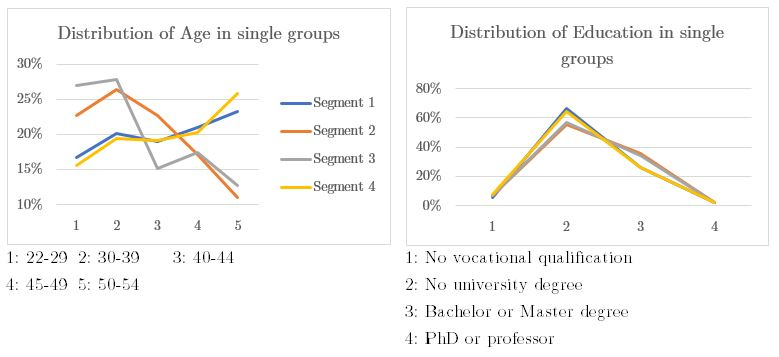
\includegraphics[width=\linewidth]{Dist1.jpg}
		\caption{(a) Distributions of the concomitant variables for the latent class analysis}
		\label{fig:DistSocioVars}
	\end{center}	
\end{figure}
\begin{figure}[H]
	\begin{center}
		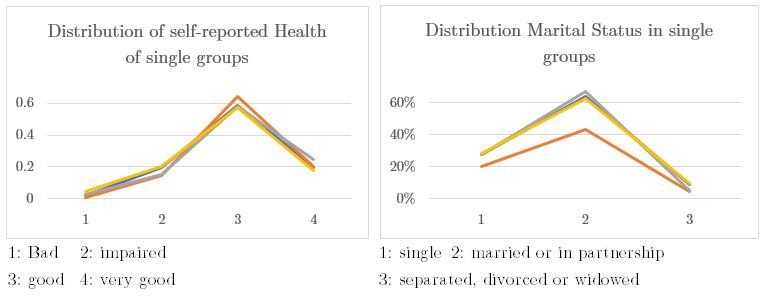
\includegraphics[width=\linewidth]{Dist2.jpg}
		\caption*{(b) Distributions of the concomitant variables for the latent class analysis}
		\label{fig:DistSocioVars}
	\end{center}	
\end{figure}
\begin{figure}[H]
	\begin{center}
		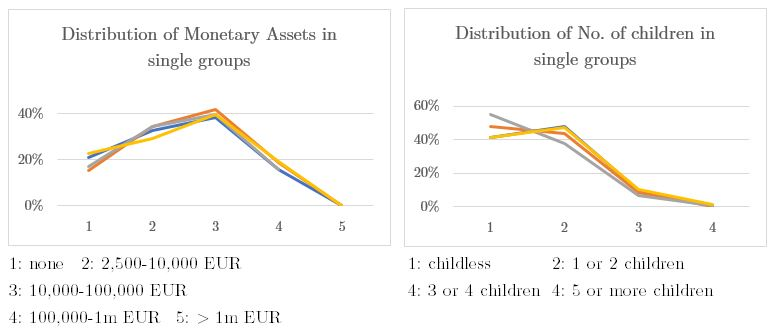
\includegraphics[width=\linewidth]{Dist3.jpg}
		\caption*{(c) Distributions of the concomitant variables for the latent class analysis}
		\label{fig:DistSocioVars}
	\end{center}	
\end{figure}
\begin{figure}[H]
	\begin{center}
		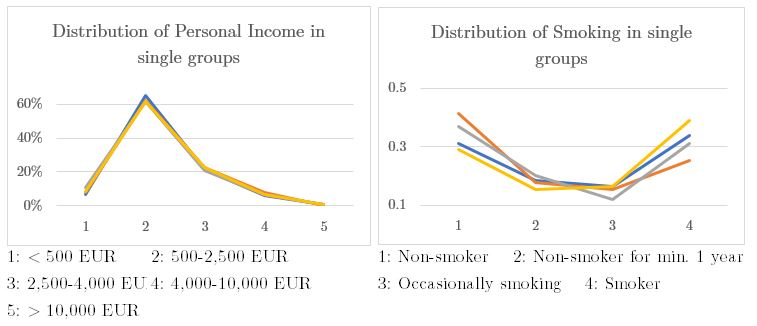
\includegraphics[width=\linewidth]{Dist4.jpg}
		\caption*{(d) Distributions of the concomitant variables for the latent class analysis}
		\label{fig:DistSocioVars}
	\end{center}	
\end{figure}
\subsection{Example of a choice set}
	\begin{figure}[H]
		\begin{center}
	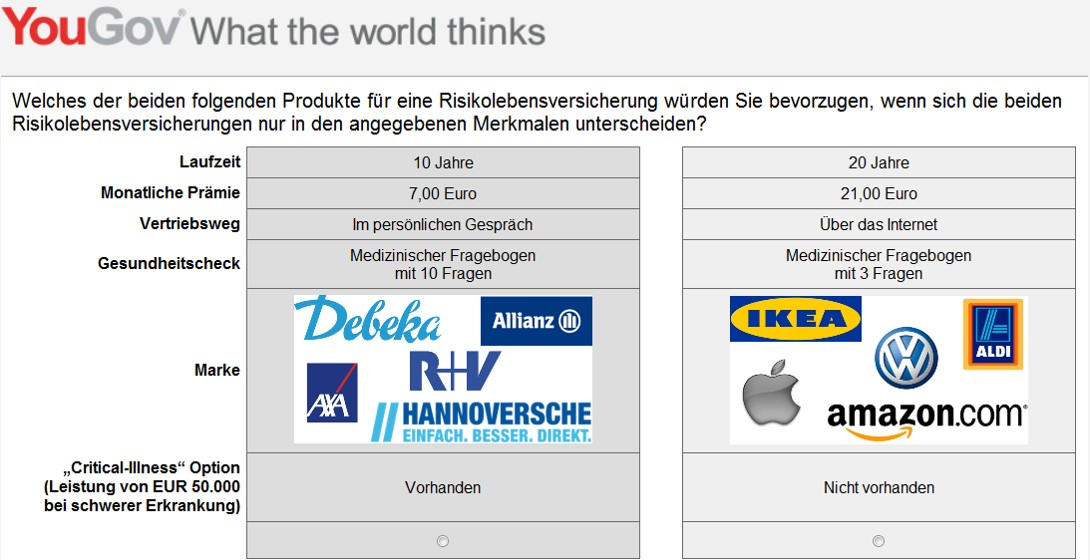
\includegraphics[width=\linewidth]{ChoiceSet_Example_NonSmoker4044.jpg}
		\caption{Choice set example for a Non-Smoker aged 40-44.}
		\label{fig:choiceset_ex}
	\end{center}	
	\end{figure}
\cleardoublepage
\section*{Statutory Declaration}
\onehalfspacing
\addcontentsline{toc}{section}{Statutory Declaration}
I hereby declare that the thesis with title
\begin{quoting}[font=itshape]
Heterogeneous preferences for term life insurance: A latent class analysis for the segmentation of the population groups in Germany
\end{quoting}
has been composed by myself autonomously and that no means other than those declared were used. In every single case, I have marked parts that were taken out of published or unpublished
work, either verbatim or in a paraphrased manner, as such through a quotation.\\
%\mbox{}\\
This thesis has not been handed in or published before in the same or similar form.\\
\mbox{}\\
\mbox{}\\
\noindent\begin{tabular}{ll}
Zurich, April 20, 2017~~~~~~~~~~~~~~~~~~~~~ & \makebox[2.5in]{\hrulefill}\\
 & (Signature)\\[60ex]
\end{tabular}
\end{document}